\documentclass[tikz,border=8pt]{standalone}
\usepackage{amsmath,amssymb}
\usepackage{tikz}
\usetikzlibrary{trees}

\begin{document}
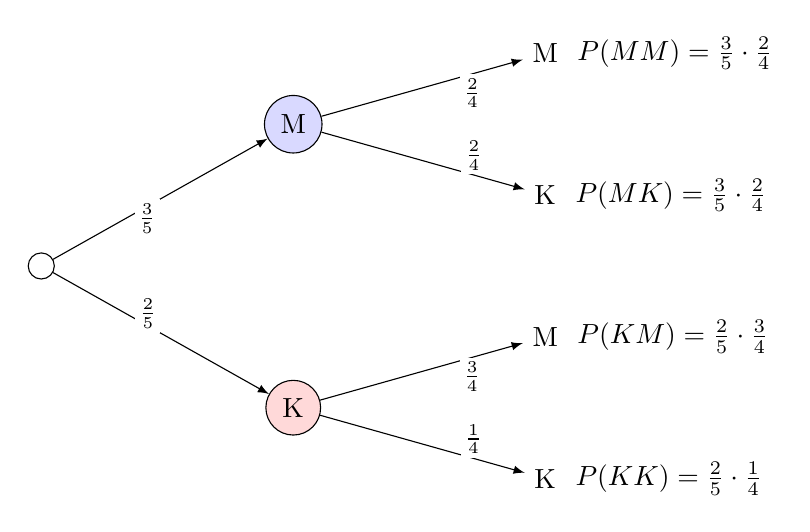
\begin{tikzpicture}[
  grow=right,
  level 1/.style={sibling distance=3.6cm, level distance=3.2cm},
  level 2/.style={sibling distance=1.8cm, level distance=3.2cm},
  edge from parent/.style={draw, -latex},
  prob/.style={fill=white, inner sep=1.5pt, font=\small},
]
  \node[circle, draw] {}
    child { node[circle, draw, fill=red!15] {K}
      child { node[label=right:{$P(KK)=\frac{2}{5}\cdot\frac{1}{4}$}] {K}
        edge from parent node[prob, above, near end] {$\frac{1}{4}$} }
      child { node[label=right:{$P(KM)=\frac{2}{5}\cdot\frac{3}{4}$}] {M}
        edge from parent node[prob, below, near end] {$\frac{3}{4}$} }
      edge from parent node[prob, above left] {$\frac{2}{5}$} }
    child { node[circle, draw, fill=blue!15] {M}
      child { node[label=right:{$P(MK)=\frac{3}{5}\cdot\frac{2}{4}$}] {K}
        edge from parent node[prob, above, near end] {$\frac{2}{4}$} }
      child { node[label=right:{$P(MM)=\frac{3}{5}\cdot\frac{2}{4}$}] {M}
        edge from parent node[prob, below, near end] {$\frac{2}{4}$} }
      edge from parent node[prob, below left] {$\frac{3}{5}$} };
\end{tikzpicture}
\end{document}
